\chapter{Asking Texas Millionaires How They Got RICH!}

This chapter follows a School of Hard Knocks interview, curated by LazyingArt LLC, but we read it as a structured lecture on wealth rather than as a parade of luxury objects. The speaker begins with spectacle, then immediately asks what stands behind it. From there the discussion unfolds in a deliberate order: first the affluent field, then leverage and mentorship, then the distinction between being broke and being poor, then a finite-life model, then a demand-shock business case, then faith and discipline, and finally a compact theory of leadership and corporate wealth. The mathematics is light, but it is not ornamental. We are given a distribution, a ribbon from \(1\) to \(100\), a scale jump, a staged planning horizon, and a final set of identities that compress the lecture's closing claims.

\section{Wealth Field and the Interview Method}

The lecture does not open by defining wealth. It points at wealth. A G-Wagon, executive biography, and a visibly affluent neighborhood are allowed to do the first bit of work. But that opening would remain merely aspirational if the lecture did not immediately formalize the setting. It does so by naming Highland Park as one of the wealthiest cities in the United States and by placing a histogram on the screen.

The visible labels in the chart are simple:
\begin{equation}
x=\text{household income }(\$1000),\qquad
y=\text{households}.
\end{equation}
We therefore introduce the notation
\begin{align}
I &\in \{10,20,30,40,50,60,75,100,125,150,200,>200\},\\
H(I) &= \text{household count in income bin } I.
\end{align}
The smaller bins are only partly legible, so the set of bins should be read conservatively. The distributional message, however, is unmistakable: the terminal \(>200\) bin dominates the display. This is a right-heavy income field.

The lecture's opening numerical claim can then be recorded as
\begin{equation}
\text{Highland Park rank}=6.
\end{equation}
That line is not mathematically sophisticated, but it performs an essential structural task. We are not being shown isolated success stories in an unspecified place. We are entering a field with unusually high local concentration of wealth.

\begin{figure}[h]
\centering

\includegraphics[width=0.86\textwidth]{lecture_88_figure_02.png}
\caption{Highland Park introduction with an overlaid income-distribution graphic. The screenshot is important because it keeps the spoken claim about local wealth tied to visible quantitative evidence and to the surrounding interview environment.}
\end{figure}

The screenshot should remain in the chapter because the lecture is doing two things at once. It is preserving the physical setting---cars, storefronts, and the highly curated public face of affluence---while also overlaying a quantitative interpretation of that setting. The chart does not replace the scene; it interprets it.

For clarity on the page, we also redraw the chart schematically. The redraw is intentionally approximate. It preserves the axes, the rough bins, and above all the dominant terminal bar, but it does not pretend to know exact counts from the frame alone.

\begin{figure}[h]
\centering
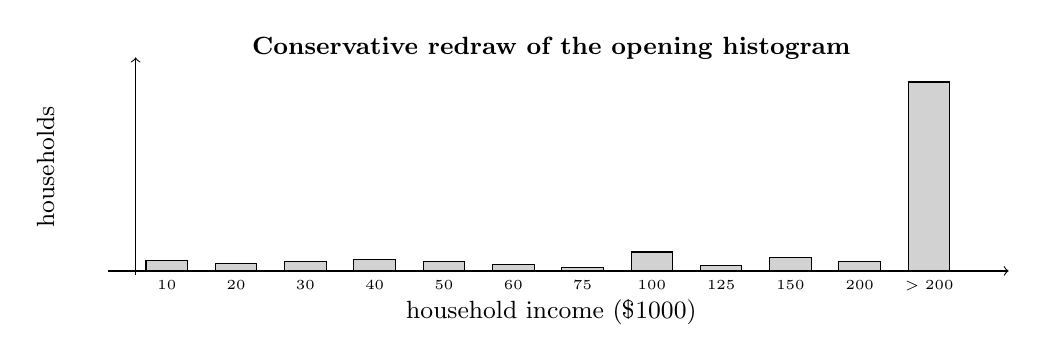
\begin{tikzpicture}[x=0.88cm,y=0.12cm]
\draw[->] (-0.4,0) -- (12.6,0);
\draw[->] (0,-0.4) -- (0,22.6);

\draw[fill=gray!35] (0.15,0) rectangle (0.75,1.1);
\draw[fill=gray!35] (1.15,0) rectangle (1.75,0.8);
\draw[fill=gray!35] (2.15,0) rectangle (2.75,1.0);
\draw[fill=gray!35] (3.15,0) rectangle (3.75,1.2);
\draw[fill=gray!35] (4.15,0) rectangle (4.75,1.0);
\draw[fill=gray!35] (5.15,0) rectangle (5.75,0.7);
\draw[fill=gray!35] (6.15,0) rectangle (6.75,0.4);
\draw[fill=gray!35] (7.15,0) rectangle (7.75,2.0);
\draw[fill=gray!35] (8.15,0) rectangle (8.75,0.6);
\draw[fill=gray!35] (9.15,0) rectangle (9.75,1.4);
\draw[fill=gray!35] (10.15,0) rectangle (10.75,1.0);
\draw[fill=gray!35] (11.15,0) rectangle (11.75,20.0);

\node[below] at (0.45,0) {\tiny 10};
\node[below] at (1.45,0) {\tiny 20};
\node[below] at (2.45,0) {\tiny 30};
\node[below] at (3.45,0) {\tiny 40};
\node[below] at (4.45,0) {\tiny 50};
\node[below] at (5.45,0) {\tiny 60};
\node[below] at (6.45,0) {\tiny 75};
\node[below] at (7.45,0) {\tiny 100};
\node[below] at (8.45,0) {\tiny 125};
\node[below] at (9.45,0) {\tiny 150};
\node[below] at (10.45,0) {\tiny 200};
\node[below] at (11.45,0) {\tiny $>200$};

\node[below] at (6,-2.0) {\small household income (\$1000)};
\node[rotate=90] at (-1.3,11) {\small households};
\node at (6,23.6) {\small \textbf{Conservative redraw of the opening histogram}};
\end{tikzpicture}
\caption{Schematic redraw of the income-distribution insert. The exact counts are not recoverable from the frame, but the heavily weighted terminal bin is clear.}
\end{figure}

Now, with the field quantified, the lecture settles into its method. Each interview is asked through a recurring sequence:
\begin{itemize}
\item What do you do?
\item How much have you made?
\item What happened in the year of peak earnings?
\item Have you ever been broke?
\item What would you tell someone younger?
\end{itemize}
That repeated template is important. It lets the lecture compare different lives without flattening them into the same story.

\section{Finance, Leverage, and the Price of Isolation}

The first executive answer gives the lecture immediate scale. The speaker says he pursued finance, had led major companies, and once made
\begin{equation}
M_{\max}=\$16.7\,\text{million}
\end{equation}
in a single year. A second interviewee later contributes another figure,
\begin{equation}
M_{\text{other}}=\$650{,}000,
\end{equation}
which the host explicitly frames as above what most people will ever make in a year. The point of placing these numbers so early is not to turn the lecture into income voyeurism. It is to establish that the subsequent principles are being spoken from within a serious range of outcomes.

From there the lecture shifts from biography to mechanism. One of its cleanest claims is that isolated labor does not scale well. Hiring creates leverage:
\begin{equation}
\text{hiring} \rightarrow \text{leverage} \rightarrow \text{scale}.
\end{equation}
This is not a theorem, but it is a true structural compression of the lecture's advice. The point is not simply that more people do more work. The point is that a person trapped within his own understanding and his own hours can only grow linearly, whereas leverage changes the geometry of growth.

\subsection{Question \& Answer}

\paragraph{Question.} Is there a shortcut to real dreams?

\paragraph{Answer.} The lecture's answer is subtle. There is no shortcut in the sense of a free bypass of work, but there is a shortcut in the sense of reducing avoidable error. Mentorship enters precisely here. It shortens the path not by suspending effort, but by compressing wasted motion.

The schematic relation is
\begin{equation}
\text{mentorship} \rightarrow \text{fewer mistakes} \rightarrow \text{shorter path}.
\end{equation}
The transcript is noisy in this passage, but the argumentative structure is clear enough to preserve. Once success has been established, the lecture naturally asks whether the path can be made straighter. The answer is yes, but only through guided correction rather than through fantasy.

This is a decisive shift. We are no longer merely asking what rich people own. We are asking what changes the rate at which a life can move.

\section{Broke, Poverty, and the Ribbon of Time}

At precisely the moment when the lecture risks becoming a list of financial tactics, it changes scale. One speaker says you can fix broke, but you cannot fix poverty. The distinction matters enough to state explicitly.

\begin{definition}
Within the local vocabulary of the lecture, \emph{broke} names a temporary condition of financial depletion, whereas \emph{poverty} names a mindset that prevents recovery and initiative.
\end{definition}

This distinction prepares the lecture for its most memorable construction. A speaker, now \(57\) years old, asks for a moment and produces a strip marked from \(1\) to \(100\). The averages he uses are
\begin{align}
A_f &= 81, &
A_m &= 75, &
a &= 57.
\end{align}
At first we may take the male average as a benchmark, in which case the nominal remainder is
\begin{equation}
R_{\text{nominal}}=A_m-a=75-57=18.
\end{equation}
The lecture then tears the ribbon. This is the crucial move. It makes lived time irrecoverable in a physical way. What is past is torn away. What remains is short enough to be held in the hand.

\subsection{Question \& Answer}

\paragraph{Question.} What, exactly, is the ribbon meant to show?

\paragraph{Answer.} It is meant to convert an abstract truth into a manipulable object. We all know, in a loose verbal sense, that life is finite. The ribbon makes finitude visible and local. It lets us compare total span, current age, and remaining segment without rhetorical fog.

The lecture then adds an important qualification. Even the nominal remainder overstates what is truly available, because future years are not uniform in quality. Illness and physical decline can compress usable life before the endpoint. A cautious mathematical rendering is therefore
\begin{equation}
R_{\text{effective}} \le R_{\text{nominal}}.
\end{equation}
This inequality is not written on the screen, but it is the correct form of the spoken argument. The point is not merely that there are \(18\) nominal years to the male-life-expectancy marker; the point is that the usable, vigorous, decision-rich segment may be smaller.

\begin{figure}[h]
\centering
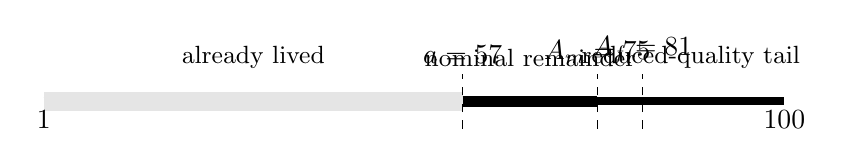
\begin{tikzpicture}[x=0.095cm,y=1cm]
\draw[line width=3pt] (1,0) -- (100,0);
\fill[gray!20] (1,-0.12) rectangle (57,0.12);
\draw[line width=4pt] (57,0) -- (75,0);
\draw[line width=1.2pt,densely dashed] (75,0) -- (100,0);

\draw[dashed] (57,-0.35) -- (57,0.35);
\draw[dashed] (75,-0.35) -- (75,0.35);
\draw[dashed] (81,-0.35) -- (81,0.35);

\node[above] at (57,0.35) {$a=57$};
\node[above] at (75,0.35) {$A_m=75$};
\node[above] at (81,0.35) {$A_f=81$};

\node[below] at (1,0) {$1$};
\node[below] at (100,0) {$100$};

\node at (29,0.55) {\small already lived};
\node at (66,0.55) {\small nominal remainder};
\node at (87.5,0.55) {\small reduced-quality tail};
\end{tikzpicture}
\caption{Transcript-based reconstruction of the ribbon demonstration. The dashed tail is not an exact calculation; it represents the lecture's insistence that nominal years and usable years are not identical.}
\end{figure}

Once this model has been introduced, the lecture can no longer be read as mere aspiration. It has turned time itself into the central scarce variable. From that point onward, business advice is forced to answer to mortality.

\section{Opportunity Shock: From \$1.5 Million to \$16.7 Million}

The lecture now returns from the ribbon to business, but it returns with more gravity. The next case is the eyeglass and hearing-aid business, and the speaker explains that a bankruptcy event at American Airlines caused workers with generous hearing-related benefits to rush toward usage while they still could.

The key numbers are
\begin{align}
M_{\text{prior}} &\approx \$1.5\,\text{million},\\
M_{\max} &= \$16.7\,\text{million},\\
N_{\text{AA}} &\approx 13{,}000.
\end{align}
The lecture's causal chain is worth preserving in worked form:
\begin{enumerate}
\item American Airlines files bankruptcy.
\item Workers fear the loss of unusually generous benefit coverage.
\item A large amount of future usage is pulled into the present.
\item Local demand for hearing services rises sharply.
\item Revenue jumps from \(M_{\text{prior}}\) to \(M_{\max}\).
\end{enumerate}
The implied scale factor is
\begin{equation}
\frac{M_{\max}}{M_{\text{prior}}}
\approx
\frac{16.7}{1.5}
\approx
11.1.
\end{equation}
That is not a small operational improvement. It is a shock-amplified step change.

So the lecture gives us another compact mechanism:
\begin{equation}
\text{bankruptcy shock} \rightarrow \text{benefit-usage surge} \rightarrow \text{revenue jump}.
\end{equation}
The point is not that one should wait around for chaos. The point is that external disorder reorders incentives and timing. A prepared business can absorb that reordering if it has capacity, courage, and enough local relevance to catch the flow.

The lecture immediately draws a second lesson from the same case. Many people, after their first taste of success, become defensive. They stop asking how to scale and start asking how not to lose what they have just won. The speaker's answer is aggressive reinvestment. Fear freezes growth; reinvestment keeps the system moving.

This is also where the lecture inserts faith. It refuses to let us misread the case as purely tactical cleverness. The speaker says his faith is inseparable from his success and from his ability to withstand hard periods when things are not okay. That spiritual note is not extraneous. It answers the same question the ribbon raised in another language: what sustains a person when the environment stops feeling safe?

\section{Discipline, Deferred Consumption, and the One--Three--Five Horizon}

The next interview returns to the visible object of desire---another G-Wagon---but again the lecture moves behind the object. A successful insurance businessman says the common trait of highly successful people is that they do not take no for an answer. That answer continues the lecture's ongoing concern with relative response. Obstacles do not vanish, but some people remain in contact with the problem longer.

Again, the lecture pairs success with previous depletion. The speaker says that at \(29\) he moved back home, had no phone, no checking account, and was broke. This is now a recurring motif: high outcome paired with earlier scarcity. The lecture is careful not to let wealth harden into static mythology. Each strong voice is made to answer for earlier fragility.

The advice to the younger self is strikingly anti-spectacular. Stay away from clubs, bottle service, and status displays that consume cash and time before they have had a chance to compound. The lecture here is not puritanical. It is chronological. Pleasure taken too early can become anti-capital. Later in the same exchange, the speaker says that having children later in life gave him less quantity of time but more quality of time. That line quietly echoes the ribbon. It is not only the amount of a resource that matters. Its structure and usability matter too.

The explicit planning device in this section is
\begin{equation}
G=\{1,3,5\}.
\end{equation}
We should read this not as an arbitrary set but as an ordered horizon:
\begin{itemize}
\item \(1\): a target near enough to be acted on now,
\item \(3\): a medium-range target at which process becomes visible,
\item \(5\): a distant enough target to hold ambition together.
\end{itemize}
The lecture's point is that goal-setting should preserve momentum. Hitting the first target should not end the motion; it should feed the next stage.

\begin{figure}[h]
\centering
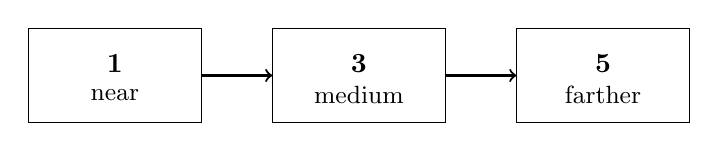
\begin{tikzpicture}
\draw (0,0) rectangle (2.2,1.2);
\draw (3.1,0) rectangle (5.3,1.2);
\draw (6.2,0) rectangle (8.4,1.2);

\node at (1.1,0.75) {\textbf{1}};
\node at (1.1,0.35) {\small near};

\node at (4.2,0.75) {\textbf{3}};
\node at (4.2,0.35) {\small medium};

\node at (7.3,0.75) {\textbf{5}};
\node at (7.3,0.35) {\small farther};

\draw[->,thick] (2.2,0.6) -- (3.1,0.6);
\draw[->,thick] (5.3,0.6) -- (6.2,0.6);
\end{tikzpicture}
\caption{Transcript-based reconstruction of the one--three--five planning horizon. The lecture uses these numbers as a simple staged scaffold for effort and motivation.}
\end{figure}

So this section gathers several strands that might otherwise seem unrelated: refusal of early discouragement, refusal of premature spectacle, quality over quantity, and the need for staged goals. The lecture is telling us that discipline is not an ornament added after success. It is one of the conditions of success.

\section{CEO Logic, Corporate Wealth, and the Meaning of Ownership}

The final interview gives the lecture its cleanest compression. The former CEO of 7-Eleven and Blockbuster says he has three things to give us: change, confidence, clarity. The transcript briefly stumbles in the middle of the triad, but the intended sequence is clear.

The first identity is the strongest:
\begin{equation}
\text{change}=\text{opportunity}.
\end{equation}
Again, this is not literal algebra. It is a rule for interpretation. Change does not feel like opportunity when it arrives. It feels like disturbance. The lecture's claim is comparative: change becomes opportunity for those who respond better than the people around them.

\subsection{Question \& Answer}

\paragraph{Question.} How does change become opportunity?

\paragraph{Answer.} Not by wishful thinking, and not automatically. It becomes opportunity when we react to the new situation faster, more accurately, or more calmly than those who merely resent it. The opportunity lies in the differential response.

From there the lecture gives us a second compressed principle:
\begin{equation}
\text{confidence}\propto \text{preparation}.
\end{equation}
This is a cautious reconstruction of the speaker's line that confidence is all about preparation. The point is that confidence should not be theatrical mood. It should be the felt consequence of having done the preparatory work.

The third term is clarity. The lecture means simplicity in explanation and definition. If strategy remains too complex to transmit, it cannot become coordinated action. That is why clarity is not cosmetic. It is operative.

\begin{figure}[h]
\centering
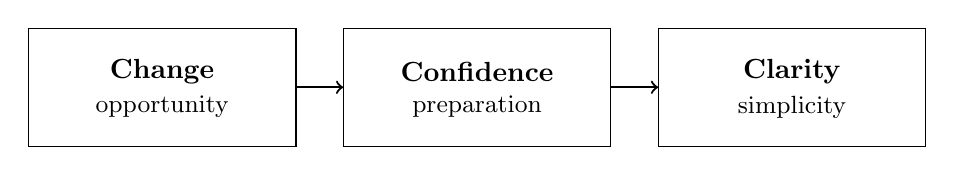
\begin{tikzpicture}
\draw (0,0) rectangle (3.4,1.5);
\draw (4,0) rectangle (7.4,1.5);
\draw (8,0) rectangle (11.4,1.5);

\node at (1.7,0.95) {\textbf{Change}};
\node at (1.7,0.50) {\small opportunity};

\node at (5.7,0.95) {\textbf{Confidence}};
\node at (5.7,0.50) {\small preparation};

\node at (9.7,0.95) {\textbf{Clarity}};
\node at (9.7,0.50) {\small simplicity};

\draw[->,thick] (3.4,0.75) -- (4,0.75);
\draw[->,thick] (7.4,0.75) -- (8,0.75);
\end{tikzpicture}
\caption{Transcript-based reconstruction of the closing triad. The lecture ends by compressing leadership into three linked motions: accept change, prepare enough to answer it with confidence, and simplify enough to lead others through it.}
\end{figure}

The lecture then makes one last important distinction. The CEO says that real corporate wealth is not primarily salary. It is ownership. So we set
\begin{align}
S &= \text{salary},\\
E &= \text{equity}.
\end{align}
Salary pays bills. It stabilizes the present. But the lecture's closing claim is
\begin{equation}
\text{wealth}_{\text{corporate}} \approx \text{equity accumulation}.
\end{equation}
This is the meaning of the SpaceX example. A person may not look rich on salary, but if that person can accumulate ownership in a repricing asset, then future wealth can detach from present cash flow. The corporate world, in the lecture's account, is built on this asymmetry.

We may summarize the closing mechanism in one final causal arrow:
\begin{equation}
\text{prepared response} \rightarrow \text{shareholder value}.
\end{equation}
That line gathers the entire final interview. Change is not enough. Preparedness is not enough. Communication is not enough. But together they convert instability into value, and equity determines whether that value sticks.

The lecture also refuses to leave this executive logic floating above the ground. It asks again whether the speaker has ever been broke, and again the answer is yes: a childhood without running water, a small shack in Massachusetts, trouble making bills at the end of the month. Even at the very end, then, the lecture preserves its recurring pattern. It does not allow success to appear detached from earlier scarcity.

\section{Summary}

We begin with spectacle, but the lecture immediately asks us to interpret the spectacle. That is why the opening chart matters. It places the interviews inside a distribution rather than inside fantasy. From there the lecture proceeds by a series of carefully motivated compressions: leverage instead of isolated labor, mentorship instead of avoidable error, a ribbon instead of a vague intuition of mortality, a demand shock instead of a lucky year, a staged goal horizon instead of undirected wanting, and equity instead of paycheck alone.

What remains on the page is not a set of disconnected slogans, though the lecture produces memorable ones. It is a sequence of formal objects and transitions. First the field. Then the mechanism. Then the limit. Then the shock. Then the discipline. Then the triad. In that order, the lecture becomes more than an interview montage. It becomes a compact theory of how wealth is perceived, built, risked, and finally interpreted.